\documentclass{article}

\usepackage{amsmath, amssymb, amsfonts}
\usepackage{tikz} % plotting
\usepackage{pgfplots}
\usepackage[dvipsnames]{xcolor} % more colors
\pgfplotsset{compat=1.18}

\usepackage{enumitem} % ordering
\usepackage[utf8]{inputenc}

% line spacing and margins
\usepackage{geometry}
\geometry{a4paper, margin=1in}

\setlength\parindent{0pt}
\linespread{1.1}
\setlength{\parskip}{0.5em}

\newcommand{\hmwkTitle}{\textbf{Homework \#2}}
\newcommand{\hmwkDueDate}{October 12, 2025}
\newcommand{\hmwkClass}{\textbf{DDA 5002 Optimization}}
\newcommand{\hmwkAuthorName}{\textbf{Xiaocao 225040374}}

\title{\hmwkClass: \hmwkTitle \\ \small Due \hmwkDueDate}
\author{\hmwkAuthorName}
\date{}

% Problem Environment
\newcounter{problemCounter}
\newenvironment{problem}[1][]{
    \refstepcounter{problemCounter}
    \vspace{1em}
    \textbf{Problem \arabic{problemCounter}} #1 \\
}{\vspace{1em}}

% Solution Environment
\newenvironment{solution}{
    \textbf{Solution:} 
}{\vspace{1em}}

\begin{document}

\maketitle

% Problem 1
\begin{problem}
\begin{solution}
    Reformulate the problem as a linear program as follows:
\begin{enumerate}[label=(\alph*)]
    \item 
\begin{align*}
\min_{x, y}\quad &  c^T x + y \\
\text{s.t.}\quad &  y \geq d^T x \\
\quad&  y \geq 0 \\
\quad&  y \geq 2 d^T x - 4\\
\quad&  Ax \geq b
\end{align*}

where $x,c,d \in \mathbb{R}^n$, $A \in \mathbb{R}^{m \times n}$, $b \in \mathbb{R}^m$, and $y \in \mathbb{R}$.


    \item 
\begin{align*}
\min_{\substack{x_1, x_2, x_3, \\ e_1, e_2, e_3}} \quad & 2 x_2 + e_1 \\
\text{s.t.} \quad &  e_1 \geq x_1 - x_3 \\
\quad & e_2 \geq x_3 - x_1 \\ 
\quad & e_2 + e_3 \leq 5\\
\quad & e_2 \geq x_1 + 2 \\
\quad & e_2 \geq -x_1 - 2 \\
\quad & e_3 \geq x_2 \\
\quad & e_3 \geq -x_2 \\
\quad & x_3 \geq - 1 \\
\quad & x_3 \leq 1 \\
\end{align*}
\end{enumerate}
\end{solution}
\end{problem}

\newpage
% Problem 2
\begin{problem}
\begin{solution} The standard form is as follows:
\begin{enumerate}[label=(\alph*)]
    \item The first problem.
\begin{align*}
\min_{x} \quad &  - x_2 + 4 x_3 - 5x_5 + 5 x_6 \\
\text{s.t.} \quad & x_1 = x_5 - x_6 \\
\quad & x_4 = - x_7 \\
\quad & x_1 + x_2 + x_3 + x_4 - x_8 = 19\\
\quad & 4 x_2 - 8 x_7 + x_9 = 45\\
\quad & 6 x_2 - x_3 + x_5 - x_6 = 7\\
\quad & x_i \geq 0, \quad i = 1, 2, \ldots, 9
\end{align*}

    \item The second problem.
\begin{align*}
\min_{x} \quad &  2x_1 - 7x_2 + 6x_3 +5x_4 \\
\text{s.t.} \quad & 2x_1 -3x_2 -5x_3 -4x_4 + x_5 = 20 \\
\quad & 7x_1 + 2x_2 + 6x_3 -2x_4 = 35 \\
\quad & 4x_1 +5x_2 -3x_3 -2x_4 - x_6 = 15 \\
\quad & x_1 + x_7 = 10 \\
\quad & x_2 + x_8 = 8 \\
\quad & x_3 - x_9 = 2 \\
\quad & x_i \geq 0, \quad i = 1, 2, \ldots, 9 \\
\end{align*}
\end{enumerate}
\end{solution}
\end{problem}

% Problem 3
\begin{problem}
\begin{solution}

\begin{center}
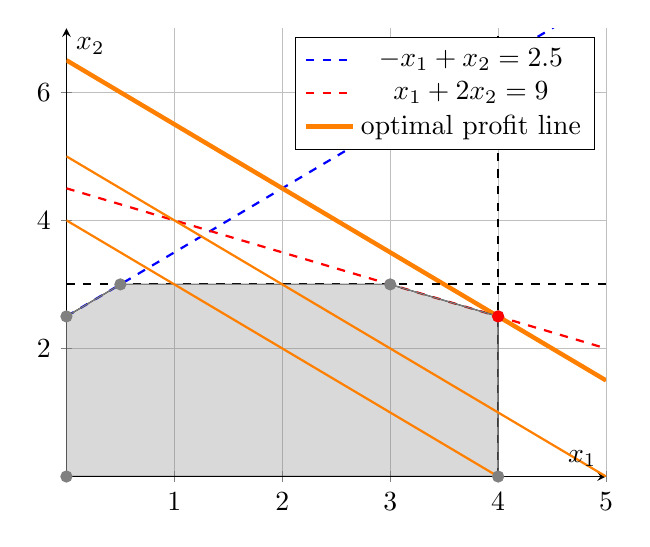
\begin{tikzpicture}
\begin{axis}[
    axis lines = middle,
    xlabel = $x_1$,
    ylabel = {$x_2$},
    grid=both,
    xmin=0, xmax=5,
    ymin=0, ymax=7,
]
\addplot [domain=0:5, blue, dashed, thick] {x + 2.5};
\addlegendentry{$-x_1 +x_2 = 2.5$}

\addplot [domain=0:5, red, dashed, thick] {-0.5*x + 4.5};
\addlegendentry{$x_1 + 2x_2 = 9$}

\addplot [domain=0:5, orange, ultra thick] {-x + 6.5};
\addlegendentry{optimal profit line}

\addplot [domain=0:5, black, dashed, thick, forget plot] {3};
\addplot [domain=0:10, black, dashed, thick] (4, x);

\addplot [fill=gray, fill opacity=0.3, draw=none, forget plot] 
    coordinates {(0,0) (0,2.5) (0.5,3) (3,3) (4,2.5) (4,0)} \closedcycle;
\addplot [black, thin, forget plot] 
    coordinates {(0,0) (0,2.5) (0.5,3) (3,3) (4,2.5) (4,0)} \closedcycle;

\addplot [mark=*, color=gray, forget plot] coordinates {(0,0) (0,2.5) (0.5,3) (3,3) (4, 2.5) (4,0)};
\addplot [mark=*, color=red, forget plot] coordinates {(4, 2.5)};

\addplot [domain=0:5, orange, thick, forget plot] {-x + 4};
\addplot [domain=0:5, orange, thick, forget plot] {-x + 5};

\end{axis}
\end{tikzpicture}
\end{center}

The graphic above shows the solution. 

The optimal value is achieved at the point (4, 2.5) with an optimal value of 6.5.

At optimal solution, the constraints $x_1 + 2x_2 \leq 9$ and $x_1 \leq 4$ are active.

All the vertices of the feasible region are (0,0), (0,2.5), (0.5,3), (3,3), (4,2.5), and (4,0).


\end{solution}
\end{problem}

\newpage
% Problem 4
\begin{problem}
\begin{solution}

Rewrite the standard form as follows:
\begin{align*}
\min_{x_1, x_2} \quad &  -x_1 -x_2 \\
\text{s.t.} \quad & x_1 +3x_2 -x_3 = 15 \\
\quad & 2x_1 + x_2 - x_4 = 10 \\
\quad & x_1 +2x_2 + x_5 = 40 \\
\quad & 3x_1 +x_2 + x_6 = 60 \\
\quad & x_i \geq 0, \quad i = 1, 2, \ldots, 6\\
\end{align*}

Denote the basic matrix as $B$, the non-basic matrix as $N$, the constants as $b$, the basic variables as $x_B$, and the non-basic variables as $x_N$.

The coefficient matrix is as follows:
\[
A = \begin{bmatrix}
1 & 3 & -1 & 0 & 0 & 0 \\
2 & 1 & 0 & -1 & 0 & 0 \\
1 & 2 & 0 & 0 & 1 & 0 \\
3 & 1 & 0 & 0 & 0 & 1 \\
\end{bmatrix}
\]

\begin{enumerate}[label=\textbf{Iter \arabic*:}]
    \item 
    Choose $\boldsymbol{x_1, x_2, x_5, x_6}$ as the initial basis.
\[
B = \begin{bmatrix}
1 & 3 & 0 & 0 \\
2 & 1 & 0 & 0 \\
1 & 2 & 1 & 0 \\
3 & 1 & 0 & 1 \\
\end{bmatrix}
\quad 
N = \begin{bmatrix}
-1 & 0 \\
0 & -1 \\
0 & 0 \\
0 & 0 \\
\end{bmatrix}
\quad
b = \begin{bmatrix}
15 \\
10 \\
40 \\
60 \\
\end{bmatrix}
\]

Solve the equations $B x_B = b$ to get the basic solution: $x_B = \bigl(3, 4, 29, 47\bigr)^T$.

Calculate the reduced cost :
$$r = c_N^T - c_B^T B^{-1} N = \bigl(0, 0\bigr) - \bigl(-1, -1, 0, 0\bigr) B^{-1} N = \bigl(-0.2, -0.4\bigr)$$

Following the smallest index rule, we choose $x_4$ as the entering variable. 

Denote the directions as $d = (d_B, d_N)$, where $d_B$ is the direction for basic variables and $d_N$ is the direction for non-basic variables; the step length as $\theta$.

\begin{align*}
d_N &= (0, 1)^T \\
d_B &= - B^{-1} N d_N = \bigl( 0.6, -0.2, -0.2, -1.6\bigr)^T \\
\theta^* &= \min_{d_{B_i} < 0} \left\{\frac{-x_{B_i}}{d_{B_i}} \right\} =  20\\
\Rightarrow x^{(1)} &= x + \theta^* d = \bigl(15,  0, 25, 15, 0, 20\bigr)^T
\end{align*}

$x_2$ leaves the basis, while $x_4$ enters.

    \item
The basis now is $\boldsymbol{x_1, x_4, x_5, x_6}$, the non-basis is $\boldsymbol{x_2, x_3}$.

\[
B^{(1)} = \begin{bmatrix}
1 & 0 & 0 & 0 \\
2 & -1 & 0 & 0 \\
1 & 0 & 1 & 0 \\
3 & 0 & 0 & 1 \\
\end{bmatrix}
\quad
N^{(1)} = \begin{bmatrix}
3 & -1 \\
1 & 0 \\ 
2 & 0 \\
1 & 0 \\   
\end{bmatrix}
\]

Solve the equations $B^{(1)} x_B = b$ to get the basic solution: $x_B^{(1)} = \bigl(15, 20, 25, 15\bigr)^T$.

Calculate the reduced cost :
$$r^{(1)} = c_N^{(1)T }- c_B^{(1)T} B^{(1)-1} N^{(1)} = \bigl(-1, 0\bigr) - \bigl(-1, 0, 0, 0\bigr) B^{(1)-1} N^{(1)} = \bigl(2, -1\bigr)$$

Following the smallest index rule, we choose $x_3$ as the entering variable.

\begin{align*}
d_N^{(1)} &= (0, 1)^T \\
d_B^{(1)} &= - B^{-1} N d_N = \bigl(1,  2, -1, -3\bigr)^T \\
\theta^{(1)*} &= \min_{d_{B_i} < 0} \left\{\frac{-x_{B_i}}{d_{B_i}} \right\} =  5\\
\Rightarrow x^{(1)} &= x + \theta^{(1)*} d = \bigl(20, 30, 20, 0, 0, 5\bigr)^T
\end{align*}

$x_6$ leaves the basis, while $x_3$ enters.
    \item
The basis now is $\boldsymbol{x_1, x_3, x_4, x_5}$, the non-basis is $\boldsymbol{x_2, x_6}$.

\[
B^{(2)} = \begin{bmatrix}
1 & -1 & 0 & 0 \\
2 & 0 & -1 & 0 \\
1 & 0 & 0 & 1 \\
3 & 0 & 0 & 0 \\
\end{bmatrix}
\quad
N^{(2)} = \begin{bmatrix}
3 & 0 \\
1 & 0 \\ 
2 & 0 \\
1 & 1 \\   
\end{bmatrix}
\]

Solve the equations $B^{(2)} x_B = b$ to get the basic solution: $x_B^{(2)} = \bigl(20, 5, 30, 20\bigr)^T$.

Calculate the reduced cost :
$$r^{(2)} = c_N^{(2)T }- c_B^{(2)T} B^{(2)-1} N^{(2)} = \bigl(-1, 0\bigr) - \bigl(-1, 0, 0, 0\bigr) B^{(2)-1} N^{(2)} = \bigl(-\frac{2}{3}, \frac{1}{3}\bigr)$$

Following the smallest index rule, we choose $x_2$ as the entering variable.

\begin{align*}
d_N^{(2)} &= (1, 0)^T \\
d_B^{(2)} &= - B^{-1} N d_N = \bigl(-\frac{1}{3}, \frac{8}{3}, \frac{1}{3}, -\frac{5}{3}\bigr)^T \\
\theta^{(2)*} &= \min_{d_{B_i} < 0} \left\{\frac{-x_{B_i}}{d_{B_i}} \right\} =  12\\
\Rightarrow x^{(2)} &= x + \theta^{(2)*} d = \bigl(16, 37, 34,  0, 12, 0\bigr)^T
\end{align*}

$x_5$ leaves the basis, while $x_2$ enters.
    \item

The basis now is $\boldsymbol{x_1, x_2, x_3, x_4}$, the non-basis is $\boldsymbol{x_5, x_6}$.

\[
B^{(2)} = \begin{bmatrix}
1 & 3 & -1 & 0 \\
2 & 1 & 0 & -1 \\
1 & 2 & 0 & 0 \\
3 & 1 & 0 & 0 \\
\end{bmatrix}
\quad
N^{(2)} = \begin{bmatrix}
0 & 0 \\
0 & 0 \\ 
1 & 0 \\
0 & 1 \\   
\end{bmatrix}
\]

Solve the equations $B^{(3)} x_B = b$ to get the basic solution: $x_B^{(3)} = \bigl(16, 12, 37, 34\bigr)^T$.

Calculate the reduced cost :
$$r^{(3)} = c_N^{(3)T }- c_B^{(3)T} B^{(3)-1} N^{(3)} = \bigl(0, 0\bigr) - \bigl(-1, -1, 0, 0\bigr) B^{(3)-1} N^{(3)} = \bigl(0.4, 0.2\bigr)$$

All the reduced costs are non-negative, so the current basic feasible solution is optimal.

So the optimal solution is $x^* = \bigl(16, 12, 0, 0, 37, 34\bigr)^T$ with an optimal value of -28. For the original problem, the optimal value is 28 with the optimal solution $x_1 = 16, x_2 = 12$.
\end{enumerate}

The feasible region and the solution at each iteration are shown in the graph below:
\begin{center}
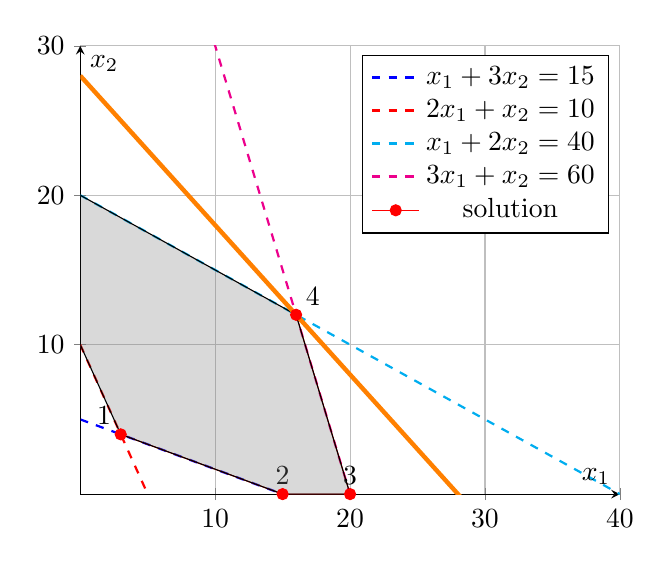
\begin{tikzpicture}
\begin{axis}[
    axis lines = middle,
    xlabel = $x_1$,
    ylabel = {$x_2$},
    grid=both,
    xmin=0, xmax=40,
    ymin=0, ymax=30,
]

\addplot [domain=0:40, blue, dashed, thick] {-x/3 + 5};
\addlegendentry{$x_1 + 3x_2 = 15$}
\addplot [domain=0:40, red, dashed, thick] {-2*x + 10};
\addlegendentry{$2x_1 + x_2 = 10$}
\addplot [domain=0:40, cyan, dashed, thick] {20 - 0.5*x};
\addlegendentry{$x_1 + 2x_2 = 40$}
\addplot [domain=0:40, magenta, dashed, thick] {60 - 3*x};
\addlegendentry{$3x_1 + x_2 = 60$}

% \addplot [mark=*, color=gray] coordinates {(3,4) (15, 0) (20,0) (16,12)};
% \addlegendentry{solution}
\addplot [mark=*, color=red] coordinates {(3,4) (15,0) (20,0) (16,12)};
\addlegendentry{solution}
\node[anchor=south east] at (axis cs:3,4) {1};
\node[anchor=south] at (axis cs:15,0) {2};
\node[anchor=south] at (axis cs:20,0) {3};
\node[anchor=south west] at (axis cs:16,12) {4};

\addplot [fill=gray, fill opacity=0.3, draw=none] 
    coordinates {(0,10) (0,20) (16,12) (20,0) (15,0) (3,4) (0,10)} \closedcycle;
\addplot [black, thin] 
    coordinates {(0,10) (0,20) (16,12) (20,0) (15,0) (3,4) (0,10)} \closedcycle;

\addplot [domain=0:40, orange, ultra thick] {-x + 28};
\end{axis}
\end{tikzpicture}
\end{center}

\end{solution}
\end{problem}

% Problem 5
\begin{problem}
\begin{solution}

\begin{enumerate}[label=(\alph*)]
    \item Denote the slack variables as $s$, the standard form of original problem is as follows:
\begin{align*}
\min_{x, s} \quad &  c_1 x_1 +c_2 x_2 +c_3x_3 + c_4x_4 \\
\text{s.t.} \quad &  x_1 -x_2 +2x_3 -s_1 = 2 \\
\quad & x_2 -x_3 +2x_4 + s_2 = 4 \\
\quad & 2x_1 +3x_3 - x_4 = 2 \\
\quad & x_i, s_j \geq 0, \quad i = 1, 2, 3, 4; j = 1, 2 \\
\end{align*}

The auxiliary LP of Phase I is as follows:
\begin{align*}
\min_{x, s, y} \quad &  y_1 +y_2 +y_3\\
\text{s.t.} \quad &  x_1 -x_2 +2x_3 \qquad-s_1 \qquad +y_1 \qquad \qquad= 2 \\
\quad & \qquad x_2 -x_3 +2x_4 \qquad+ s_2 \qquad+  y_2 \qquad = 4 \\
\quad & 2x_1 \qquad+3x_3 - x_4 \qquad \qquad \qquad \qquad+y_3 = 2 \\
\quad & x_i, s_j, y_k \geq 0, \quad i \in \mathbb{I}; j \in \mathbb{J}; k \in \mathbb{K}\\
\text{where} \quad & \mathbb{I} = \{1, 2, 3, 4\}, \mathbb{J} = \{1, 2\}, \mathbb{K} = \{1, 2, 3\}
\end{align*}

    \item 
Consider the basis with variables $x_1, x_4, y_2$.
The basis matrix and the constant vector are as follows:
\[
B = \begin{bmatrix}
1 & 0 & 0 \\
0 & 2 & 1 \\
2 & -1 & 0 \\
\end{bmatrix}
\quad
b = \begin{bmatrix}
2 \\
4 \\
2 \\
\end{bmatrix}
\]
Solve the equations $B x_B = b$ to get the basic solution: $x_B = \bigl(2, 2, 0\bigr)^T$.

Current solution is $x = \bigl(2, 0, 0, 2, 0, 0, 0, 0, 0\bigr)^T$. The auxiliary objective value is 0 and each element of $x$ is non-negative, so the current basic feasible solution is optimal for the auxiliary LP. This is the minimum value that could be achieved under the constraints, so it is optimal for the auxiliary LP of Phase I.

    \item 
The inverse of basis matrix is as follows:
\[
B^{-1} = \begin{bmatrix}
1 & 0 & 0 \\
2 & 0 & -1 \\
-4 & 1 & 2 \\
\end{bmatrix}
\]

Currently, the basis is $(x_1, x_4, y_2)$. The non-basic variables are $(x_2, x_3, s_1, s_2, y_1, y_3)$. So there are 6 possible basic directions. 

Denote each column as a possible direction of the non-basic variable entering the basis. The directions matrix for non-basic variables is the 6-dimensional identity matrix $I_6$. Denote it as $D_N$. 

For basic variables, the direction $d_B = - B^{-1} N d_N$. So we have $D_B = - B^{-1} N D_N$.

\begin{align*}
D_B
&= - B^{-1} N D_N \\
&= - B^{-1} N I_6 \\
&= - \begin{bmatrix}
1 & 0 & 0 \\
2 & 0 & -1 \\
-4 & 1 & 2 \\
\end{bmatrix}
\quad
\begin{bmatrix}
-1 & 2 & -1 & 0 & 1 & 0 \\
1 & -1 & 0 & 1 & 0 & 0 \\
0 & 3 & 0 & 0 & 0 & 1 \\
\end{bmatrix} 
\quad
\begin{bmatrix}
1 & 0 & 0 & 0 & 0 & 0 \\
0 & 1 & 0 & 0 & 0 & 0 \\
0 & 0 & 1 & 0 & 0 & 0 \\
0 & 0 & 0 & 1 & 0 & 0 \\
0 & 0 & 0 & 0 & 1 & 0 \\
0 & 0 & 0 & 0 & 0 & 1 \\
\end{bmatrix}\\
&=\begin{bmatrix}
1 & -2 & 1 & 0 & -1 & 0 \\
2 & -1 & 2 & 0 & -2 & 1 \\
-5 & 3 & -4 & -1 & 4 & -2 \\
\end{bmatrix}\\
\end{align*}

So all basic directions are shown in the matrix $D_B$, where column $i$ is the direction when the $i$-th non-basic variable enters the basis:
\[
D_B = \begin{bmatrix}
1 & -2 & 1 & 0 & -1 & 0 \\
2 & -1 & 2 & 0 & -2 & 1 \\
-5 & 3 & -4 & -1 & 4 & -2 \\
\end{bmatrix}
\]

The reduced costs:
\begin{align*}
r &= c_N^T - c_B^T B^{-1} N \\[4pt]
&= (0, 0, 0, 0, 1, 1) - (0, 0, 1)
\begin{bmatrix}
1 & 0 & 0 \\
2 & 0 & -1 \\
-4 & 1 & 2 \\
\end{bmatrix}
\quad
\begin{bmatrix}
-1 & 2 & -1 & 0 & 1 & 0 \\
1 & -1 & 0 & 1 & 0 & 0 \\
0 & 3 & 0 & 0 & 0 & 1 \\
\end{bmatrix} \\[4pt]
&= \begin{bmatrix}
-5 &  3 & -4 & -1 &  5 & -1
\end{bmatrix}
\end{align*}

Till now, not all the reduced costs are non-negative. following the smallest index rule, we choose $x_2$ as the entering variable.

\begin{enumerate}[label=\textbf{Iter \arabic*:}]
    \item $x_2$ enters, $y_2$ leaves.

\textbf{Basis:} $(x_1, x_4, x_2)$

\textbf{Non-basis:} $(y_2, x_3, s_1, s_2, y_1, y_3)$

\[
B^{(1)} = \begin{bmatrix}
1 & 0 & -1 \\
0 & 2 & 1 \\
2 & -1 & 0 \\
\end{bmatrix}
\quad
N^{(1)} = \begin{bmatrix}
0 & 2 & -1 & 0 & 1 & 0 \\
1 & -1 & 0 & 1 & 0 & 0 \\
0 & 3 & 0 & 0 & 0 & 1 \\
\end{bmatrix}
\]

\[
x_B^{(1)} = B^{(1)-1} b = \begin{bmatrix}
2 & 2 & 0
\end{bmatrix} ^T
\]

The reduced costs:
\begin{align*}
r &= c_N^{(1)T} - c_B^{(1)T} B^{(1)-1} N^{(1)} \\[4pt]
&= (1, 0, 0, 0, 1, 1) - (0, 0, 0) B^{(1)-1} N^{(1)} \\[4pt]
&= \begin{bmatrix}
1 & 0 & 0 & 0 & 1 & 1
\end{bmatrix} \\
\end{align*}
All the reduced costs are non-negative. Current optimal solution for the auxiliary LP is $x^{(1)} = \bigl(2, 0, 0, 2, 0, 0, 0\bigr)^T$ with an optimal value of $0$.
\end{enumerate}

% Due to the basis contains auxiliary variables, we need replace $y_2$ with a non-basic variable.

% Replace $y_2$ with $x_2$. The new basis matrix and non-basis matrix are as follows:
% \[
% B = \begin{bmatrix}
% 1 & 0 & -1 \\
% 0 & 2 & 1 \\
% 2 & -1 & 0 \\
% \end{bmatrix}
% \quad
% N = \begin{bmatrix}
% 2 & -1 & 0 \\
% -1 & 0 & 1 \\
% 3 & 0 & 0 \\
% \end{bmatrix}
% \]

% Compute $det(B) = 5$, so the new basic column is linearly independent with other basic columns and the new basis is valid. Take $x_1, x_2, x_4$ as the basis and the current basic feasible solution is $x_B = \bigl(2, 0, 2\bigr)^T$. The non-basic variables are $x_3, s_1, s_2$ solution is $x_N = \bigl(0, 0, 0\bigr)^T$. 

% Starting from the basis, the inverse of basis matrix is $B^{-1}$:
% \[
% B^{-1} = \begin{bmatrix}
% 0.2 &  0.2 &  0.4 \\
% 0.4 &  0.4 & -0.2 \\
% -0.8 &  0.2 &  0.4
% \end{bmatrix}
% \]

% The number of all the variables is 6, so currently there are 3 possible directions. The present basis is $(x_1, x_2, x_4)$. The non-basic variables are $(x_3, s_1, s_2)$.

% \begin{enumerate}[label=(\roman*)]
%     \item $d_N = (1, 0, 0)^T$ (entering $x_3$)
% \begin{align*}
% d_B^{(\mathrm{i})} 
% &= - B^{-1} N d_N \\[4pt]
% &= -
% \begin{bmatrix}
% 0.2 &  0.2 &  0.4 \\
% 0.4 &  0.4 & -0.2 \\
% -0.8 &  0.2 &  0.4
% \end{bmatrix}
% \begin{bmatrix}
% 2 & -1 & 0 \\
% -1 & 0 & 1 \\
% 3 & 0 & 0
% \end{bmatrix}
% \begin{bmatrix}
% 1 \\ 0 \\ 0
% \end{bmatrix}
% =
% \begin{bmatrix}
% -1.4 \\ 0.2 \\ 0.6
% \end{bmatrix}
% \end{align*}

%     \item $d_N = (0, 1, 0)^T$ (entering $s_1$)
% \begin{align*}
% d_B^{(\mathrm{ii})} 
% &= - B^{-1} N d_N \\[4pt]
% &= -
% \begin{bmatrix}
% 0.2 &  0.2 &  0.4 \\
% 0.4 &  0.4 & -0.2 \\
% -0.8 &  0.2 &  0.4
% \end{bmatrix}
% \begin{bmatrix}
% 2 & -1 & 0 \\
% -1 & 0 & 1 \\
% 3 & 0 & 0
% \end{bmatrix}
% \begin{bmatrix}
% 0 \\ 1 \\ 0
% \end{bmatrix}
% =
% \begin{bmatrix}
% 0.2 \\ 0.4 \\ -0.8
% \end{bmatrix}
% \end{align*}

%     \item $d_N = (0, 0, 1)^T$ (entering $s_2$)
% \begin{align*}
% d_B^{(\mathrm{i})} 
% &= - B^{-1} N d_N \\[4pt]
% &= -
% \begin{bmatrix}
% 0.2 &  0.2 &  0.4 \\
% 0.4 &  0.4 & -0.2 \\
% -0.8 &  0.2 &  0.4
% \end{bmatrix}
% \begin{bmatrix}
% 2 & -1 & 0 \\
% -1 & 0 & 1 \\
% 3 & 0 & 0
% \end{bmatrix}
% \begin{bmatrix}
% 0 \\ 0 \\ 1
% \end{bmatrix}
% =
% \begin{bmatrix}
% -0.2 \\ -0.4 \\ -0.2
% \end{bmatrix}
% \end{align*}
% \end{enumerate}

% Reduced costs for all the elements in $x_N$ is
% \begin{align*} 
% r &= c_N^T -c_B^T B^{-1} N
% &= (c_3, 0, 0) - (c_1, c_2, c_4) B^{-1} N \\
% &= \\
% \end{align*}


\end{enumerate}
\end{solution}
\end{problem}

% Problem 6
\begin{problem}
\begin{solution}

\begin{enumerate}[label=(\alph*)]
    \item \textbf{False.}

According to the definition of bounded set (in the real cases), a set is bounded if there exists $M \in \mathbb{R}$ such that the size of every element in the set is no more than $M$.

Take the following LP as a counter-example:
\begin{align*}
\min_{x_1, x_2, x_3} \quad &  x_1 - x_2 + x_3\\
\text{s.t.} \quad &  x_1 - x_2 + x_3 = 0 \\
\quad &  x_1, x_2, x_3 \geq 0 \\
\end{align*}

Obviously, the optimal solution exists, and the optimal value is 0. The optimal solution set is $S^* = \{x \in \mathbb{R}^3 \mid x_1 - x_2 + x_3 = 0, \textbf{x} \geq 0\}$.

Consider the optimal solution $x = (\lambda, \lambda, 0)^T \in S^* \quad\forall \lambda \geq 0$. Since $\lambda$ is unbounded, the optimal solution set $S^*$ is unbounded.

    \item \textbf{False.}
    
Take the same LP in \(a\) as a counter-example. Consider the optimal solution $x = (1, 2, 1)^T \in S^*$. This optimal solution has 3 positive components, while the rank of the coefficient matrix $m = 1$.
    \item \textbf{True.}

For the optimal set being convex, if both $x_1$ and $x_2$ are optimal solutions, then $c^T x_1 = c^T x_2$. There exists $\lambda \in [0, 1]$, $x = \lambda x_1 + (1-\lambda) x_2$, then $c^T x = \lambda c^T x_1 + (1-\lambda) c^T x_2 = c^T x_1$. So $x$ is also an optimal solution. So if there are more than one optimal solution, then there are infinite optimal solutions.
    \item \textbf{False.}

Take the same LP in \(a\) as a counter-example. Consider the optimal solution $x = (1, 2, 1)^T \in S^*$. This optimal solution has 3 positive components, while the rank of the coefficient matrix $m = 1$. It doesn't satisfy the definition of basic solution which requires at most $m$ positive components. So this optimal solution is not a basic feasible solution.
\end{enumerate}

\end{solution}
\end{problem}
\end{document}
